\subsection{Server architecture} \label{sec:serverarch}

The Anastasis server architecture consists of two components. A web
server with a REST API and a PostgreSQL database. The structure of
these two components is shown in Figure~\ref{fig:anastasis:server}.

\begin{figure}[H]
	\centering
	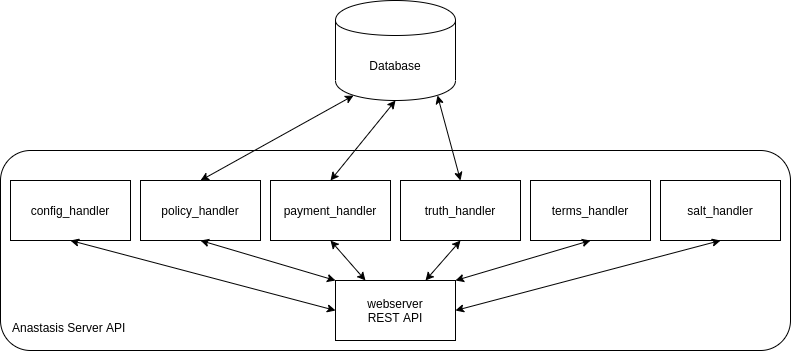
\includegraphics[scale=0.45]{images/server_api.png}
	\caption{Anastasis server architecture}
	\label{fig:anastasis:server}
\end{figure}

The webserver of Anastasis provides a RESTful API. For a detailed
documentation of the REST API, see
appendix ~\ref{appendix_server_api}.

\newpage
\subsubsection{Database}

The database schema of Anastasis is shown in
Figure~\ref{fig:anastasis_database}.
\begin{figure}[H]
	\centering
	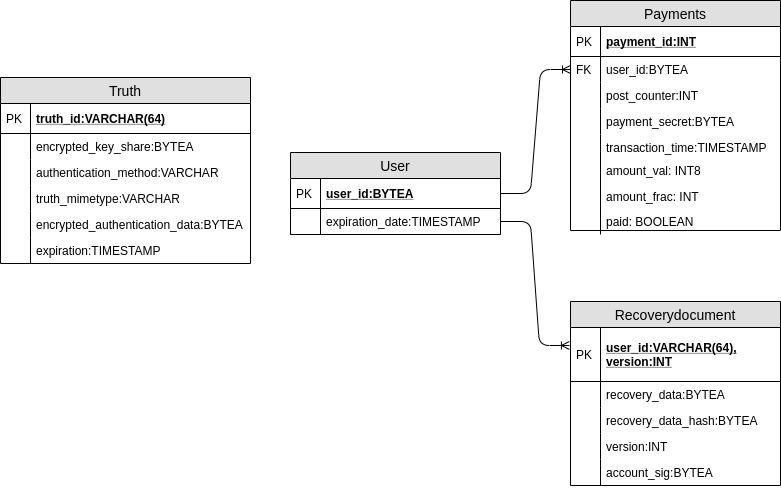
\includegraphics[scale=0.5]{images/anastasis-db.png}
	\caption{Anastasis database schema}
	\label{fig:anastasis_database}
\end{figure}

The database schema consists of four main tables:

\begin{itemize}
\item The {\em Truth} table is responsible for storing the key shares and
  its authentication method. The key share and the authentication data are stored
  encrypted in the database. The authentication data is only decrypted during
  authentication. The key share is never decrypted for the
  server. This protects the privacy of the customer. Likewise, the
  user data is protected after a possible theft.
\item The {\em User} table contains the identification of the user and an
  expiration timestamp. This timestamp is a subscription period. This
  timestamp is updated after each payment the user makes. Users for
  whom the subscription has expired are periodically deleted.
\item The {\em Payments} table contains the details of a payment from a
  user. The payment is used either for the post-counter or the
  subscription. The post-counter is decremented after each upload of a
  recovery document. The user can only upload the recovery document if
  the provided payment contains a post-counter which is at least 1.
  Through this measure we can prevent people from maliciously filling
  our database.
\item The {\em Recoverydocument} table contains the recovery
  information. The recovery document is stored encrypted in the
  database. This offers better protection, as explained earlier for
  the Truth table. Each recovery document record also contains a
  version, a hash of the recovery document and a signature. The
  version attribute allows the user to lookup a specific version of
  the document. The hash is used to check if the user uploads a
  duplicate of the document. The signature attests the
  integrity of the recovery data.
\end{itemize}


\subsubsection{Authentication methods}

This section describes an overview over the different possible
authentication methods for Anastasis. In our implementation only the
secure question is implemented. The other methods are just explained
how they would be implemented.

In all cases, the authentication process begins by the user decrypting
their (encrypted) recovery document, which contains a list of Anastasis
providers, associated authentication methods, truth\_seeds and associated
truth encryption keys.  The recovery process than varies slightly
depending on the authentication method.

\paragraph{SMS (sms)}

The user tells the server with a request that they wants to authorize
key recovery (via GET /truth/\$TRUTH\_PUB), providing a way to decrypt the
truth with the phone number. The server will then generate a \$PIN and
send it via an SMS provider to the stored number in the truth
object. The client then must send another request with the sent \$PIN
(via GET /truth/\$TRUTH\_PUB?response=\$PIN). The server can now check
if the two PINs match. Upon success, the server returns the encrypted
key share.

\paragraph{Video identification (vid)}

This method allows the user to identify via video-call.  Since the
respective images must be passed on to the video identification
service in the event of password recovery, it must be ensured that no
further information about the user can be derived from them.  Hence,
the user's client software must try to delete metadata that could
result in accidental information leakage about the user from the image
before encrypting and uploading it to the Anastasis provider.

For recovery, the user must first send a request to server that they
wants to authorize recovery (GET /truth/\$TRUTH\_PUB).  The Anastasis
provider will then decrypt the user's image and send a request with a
\$TOKEN to a video authentication provider that a user wants to
authenticate, and respond to the user with a link to a video
conference.  The video authentication provider then checks via video
conference that the user in the image is the same that they have on
the video link. Upon success, the video provider releases the \$TOKEN
to the user.  The client then must send another request with the
\$TOKEN (via GET /truth/\$TRUTH\_PUB?response=\$TOKEN). The Anastasis
provider checks that the tokens match, and upon success returns the
encrypted key share.

\paragraph{Post identification (post)}

The user tells the Anastasis provider with a request that they want
to authenticate using Post identification (GET /truth/\$TRUTH\_PUB).  The
Anastasis provider uses the request to decrypt the user's truth to
determine the user's postal address, and sends them letter containing
a \$PIN.  Upon receiving the letter, the client then has to send
another request with the \$PIN (GET /truth/\$TRUTH\_PUB?response=\$PIN). The
server can now check if the two PINs match. Upon success the server
will release the encrypted key share.

\paragraph{Security question (qa)}

The user provided Anastasis with a secure question and a (normalized)
answer.  The secure question becomes part of the encrypted recovery
document, and is never disclosed to weak adversaries, even during
recovery.  The encrypted truth on the server only contains a (salted)
hash of the answer. The Anastasis provider cannot learn the plaintext
answer. Because of the salt, and it cannot mount a confirmation attack
either.

If the user wants to recover the key share from the server, they must
provide the (salted) hash of the answer to the security question (via
GET /truth/\$TRUTH\_PUB?response=\$HASH). The server then checks if the
stored and the provided hash match. Upon success the server responds
with the encrypted key share.
